\documentclass[10pt,twocolumn,letterpaper]{article}

\usepackage{acvs}
\usepackage{times}
\usepackage{epsfig}
\usepackage{graphicx}
\usepackage{amsmath}
\usepackage{amssymb}

% Include other packages here, before hyperref.
\usepackage{dsfont}

% If you comment hyperref and then uncomment it, you should delete
% egpaper.aux before re-running latex.  (Or just hit 'q' on the first latex
% run, let it finish, and you should be clear).
\usepackage[pagebackref=true,breaklinks=true,letterpaper=true,colorlinks,bookmarks=false]{hyperref}

\iccvfinalcopy % *** Uncomment this line for the final submission

\def\iccvPaperID{} % *** Enter the Paper ID here
\def\httilde{\mbox{\tt\raisebox{-.5ex}{\symbol{126}}}}

% Pages are numbered in submission mode, and unnumbered in camera-ready
\ificcvfinal\pagestyle{empty}\fi

\begin{document}

%%%%%%%%% TITLE - PLEASE UPDATE
\title{CenterFormer: Center-based Transformer for 3D Object Detection~\cite{centerformer} \\ {\rm {\normalsize Minji Kim (minji@snu.ac.kr; 2020-28702), Dept. of Electrical and Computer Engineering, Seoul National University}}}   % **** Enter the paper title and student information here

\maketitle
\thispagestyle{empty}

%%%%%%%%% BODY TEXT - ENTER YOUR RESPONSE BELOW

%%%%%%%%%%%%%%%%%
%%%%%%%%%%%%%%%%%
\section{Introduction}
Inspired by DEtection Transformer (DETR)~\cite{detr}, this paper investigates a novel center-based Transformer for 3D object detection named CenterFormer.
In DETR-style encoder-decoder transformer network, the computational complexity grows quadratically when input size increases.
Thus, directly using the Transformer encoder on voxel or Bird Eye View (BEV) feature map is impractical due to its large size.
For the efficiency and effectiveness in learning the DETR-style networks, this paper proposes to use the center feature as the initial query embedding to capture the object-centric information.
Furthermore, the cross-attention learning based on a small multi-scale window is also helpful for reducing the computational complexity.
Results on Waymo Open Dataset shows that CenterFormer reaches state-of-the-art performance with multi-frame extension.



%%%%%%%%%%%%%%%%%
%%%%%%%%%%%%%%%%%
\section{CenterFormer}

Fig.~\ref{fig:overview} shows the overall architecture of CenterFormer.
The network consists of four parts: a voxel feature encoder that encodes the raw point cloud into a BEV feature representation, a multi-scale center proposal network (CPN), the center-based transformer decoder, and a regression head that predicts the bounding box.
First, the point cloud is encoded into a BEV function representation using a standard voxel-based backbone network.
Next, the feature map is transformed to different scales, followed by a multi-scale center proposal network to predict the initial center position.
The proposed center feature is utilized as the input for the transformer encoder as query embedding.
Like Deformable DETR~\cite{deformabledetr}, a deformable cross attention layer is adopted in each Transformer module for the effective aggregation of multi-scale feature maps.
Finally, the output object representation is regressed to other object properties to produce the final object prediction.




%%%%%%%%%%%%%%%%%
%%%%%%%%%%%%%%%%%
\section{Experiments}

\paragraph{Results}
Experimental results are summarized in Fig.~\ref{fig:experiment}, surpassing other methods in terms of Mean L2, although using multi-frame settings in comparison with other methods with single frame setting seems unfair for me.

\paragraph{Difference with Deformable DETR}
This paper is largely inspired by Deformable DETR~\cite{deformabledetr}. However, the difference between CenterFormer and Deformable DETR can be summarized as follows:
\begin{itemize}
\item CenterFormer only adopts decoder part of Transformers.
\item Center feature is used as the query embedding instead of the learnable parameters.
\item The set matching strategy is not adopted since it is hard to converge~\cite{yin2021center}
\end{itemize}
These features help the CenterFormer to train and test effectively and robustly in the task of 3D object detection.



\begin{figure}[t]
    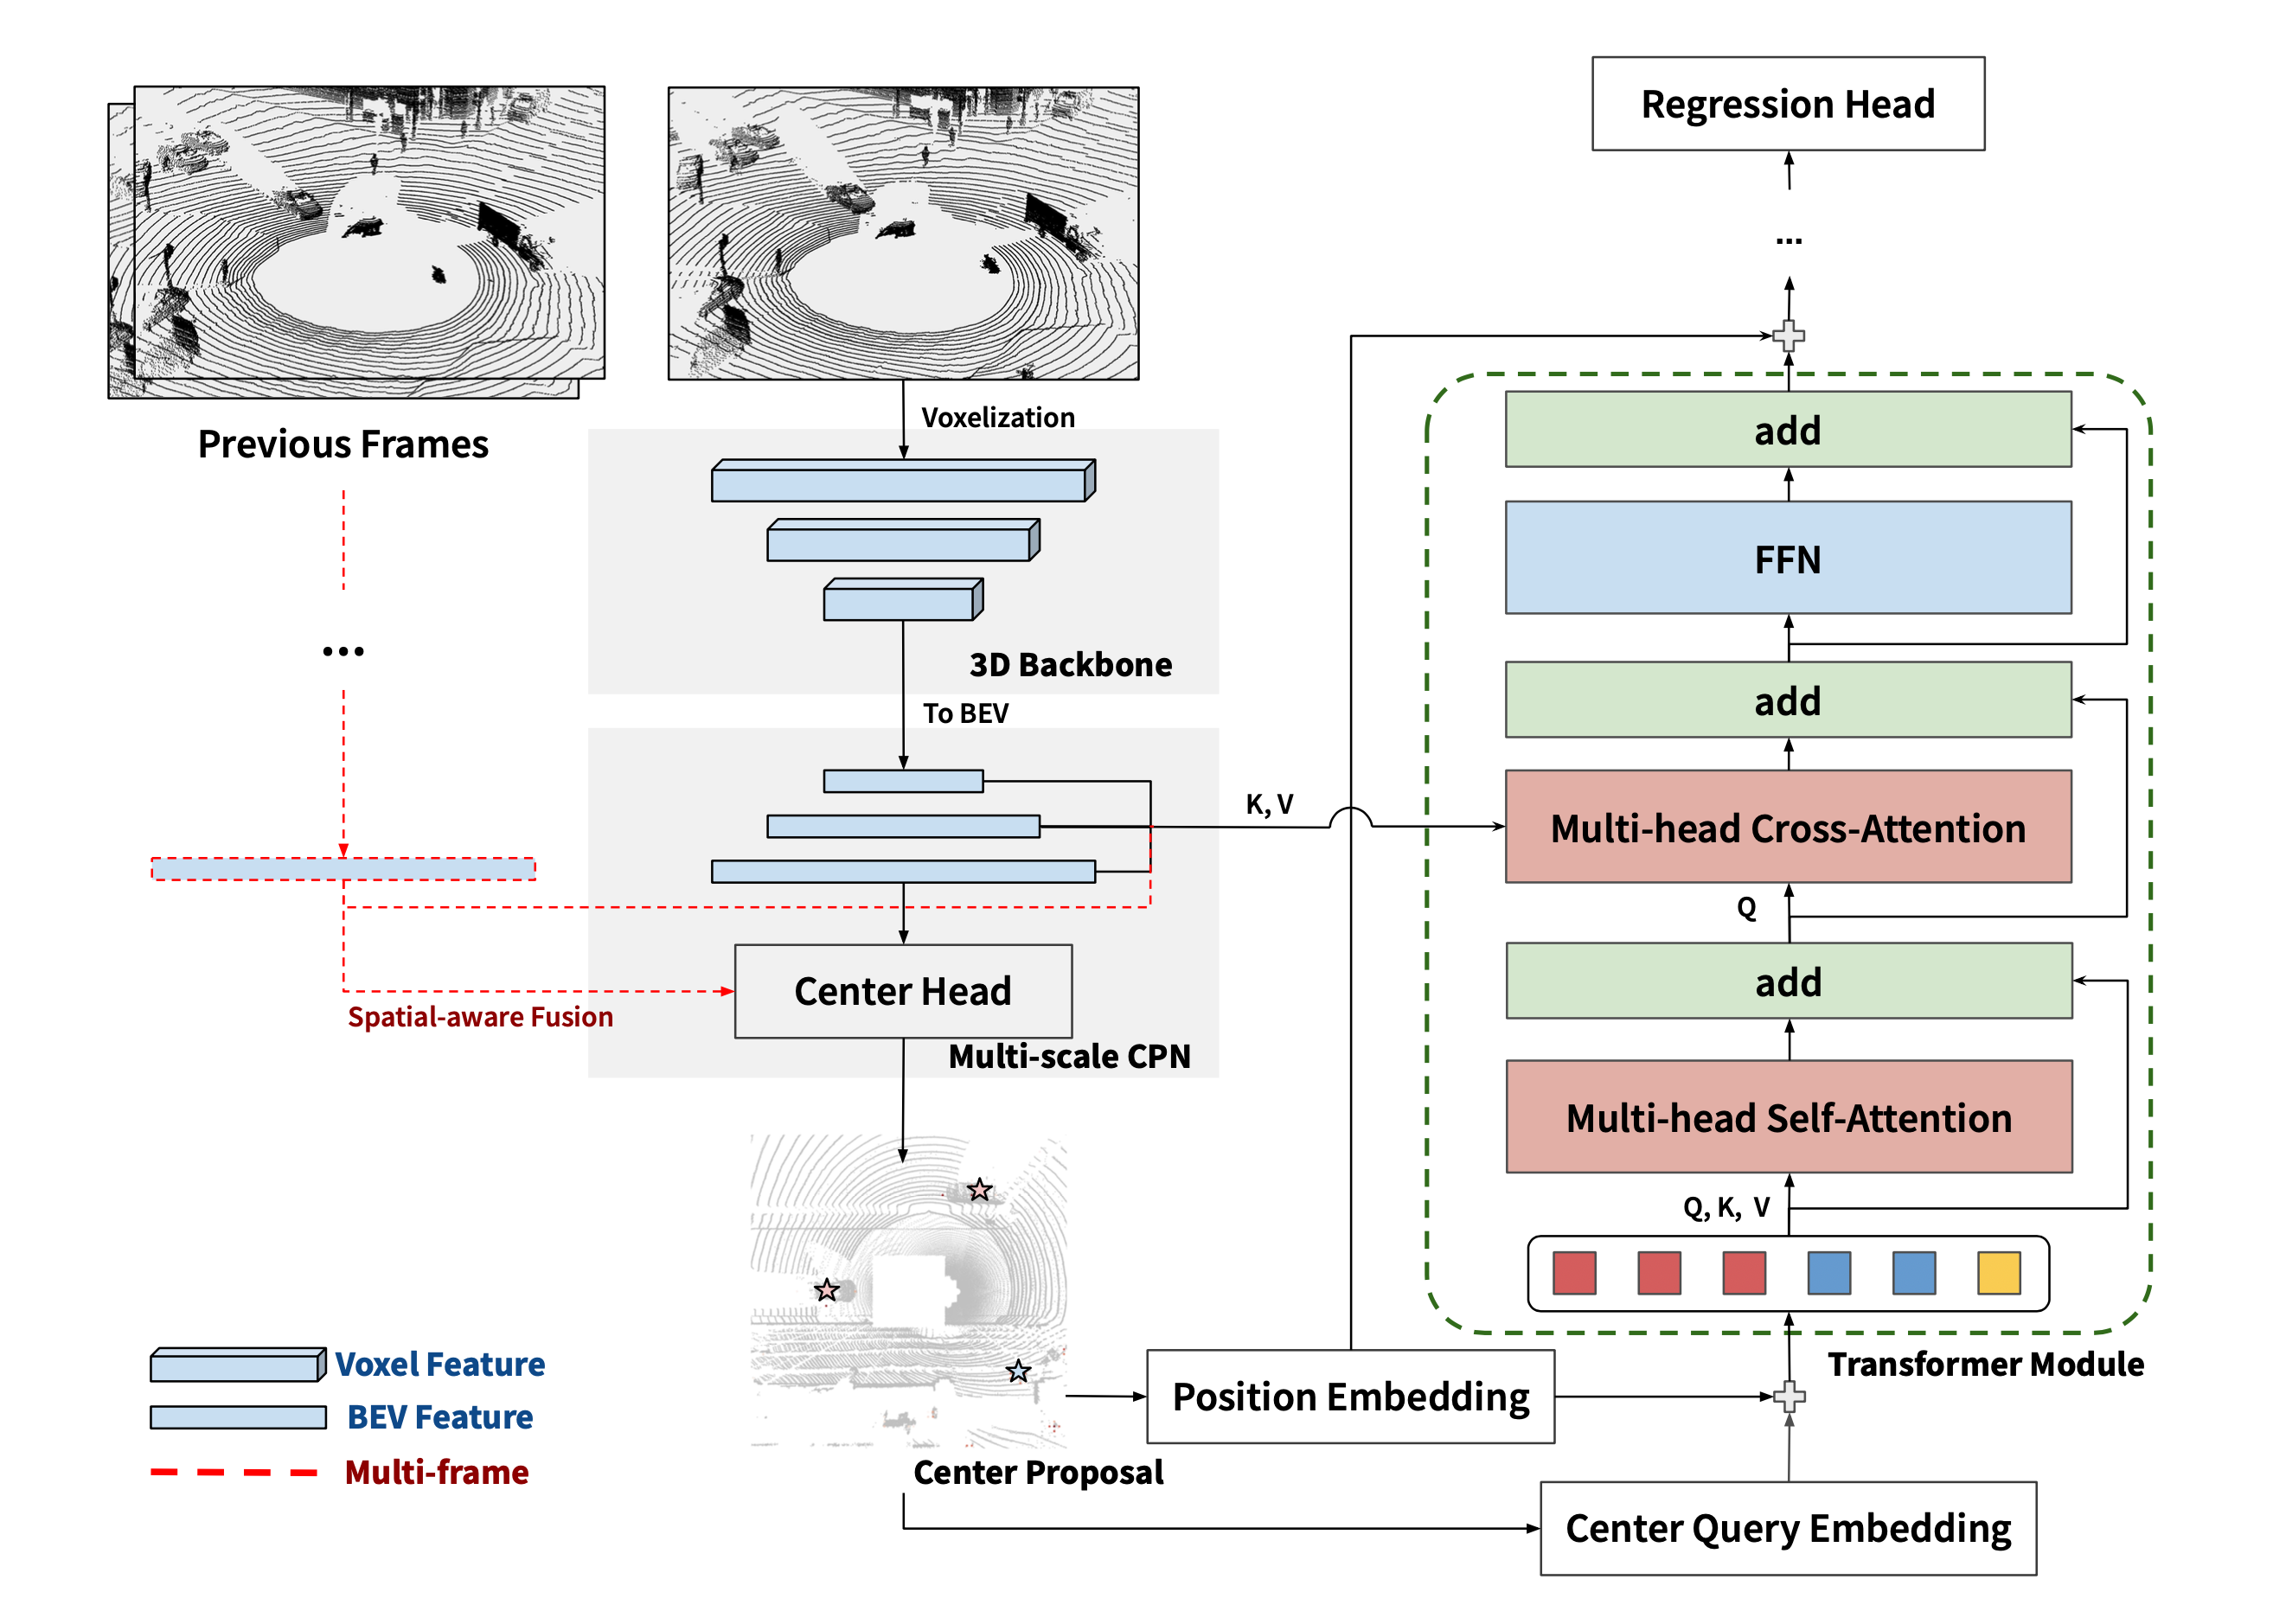
\includegraphics[width=\linewidth]{assets/centerformer.png}
    \caption{\label{fig:overview}The overall pipeline of CenterFormer.}
\end{figure}

\begin{figure}[t]
    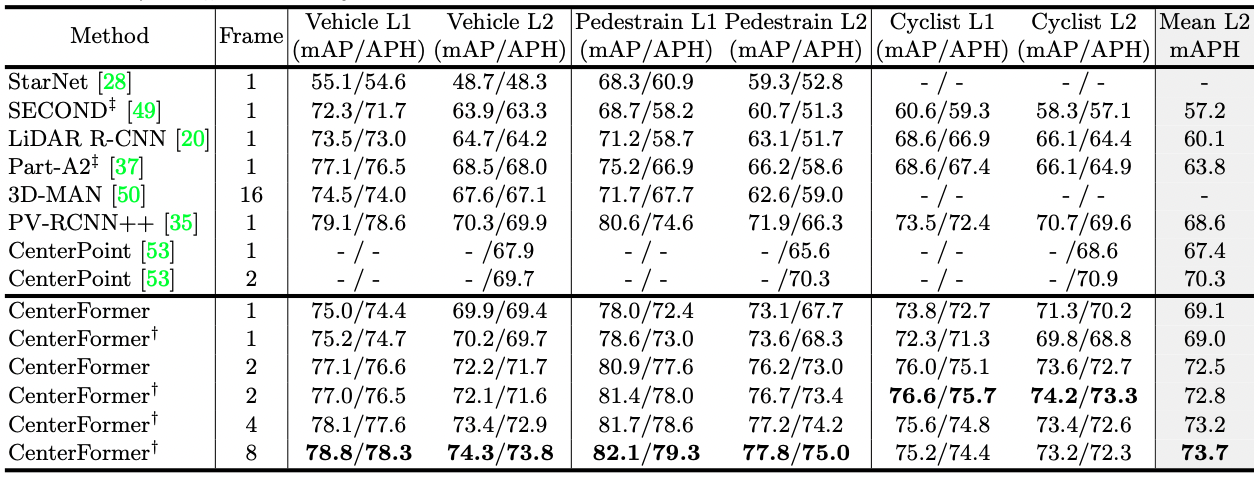
\includegraphics[width=\linewidth]{assets/experiment.png}
    \caption{\label{fig:experiment}The overall pipeline of CenterFormer.}
\end{figure}



{\small
\bibliographystyle{ieee}
\bibliography{egbib}
}

\end{document}
